\subsection{Manipulador com base esférica}
Um projeto de pesquisa e desenvolvimento foi apresentado em
\cite{motta2010prototype} com o objetivo de propor metodologia, simulação e
os passos para construção de um sistema robótico para recuperar danos materiais
em pás de turbinas hidráulicas gerados devido à cavitação. O sistema robótico faz
reparo utilizando a tecnologia de soldagem a arco elétrico, antes realizada
manualmente em ambientes de alta periculosidade com temperaturas que variam
entre $40^o C$ e $99^o C$ em operações que duram em torno de 10 horas. 

O robô deve atender aos seguintes requisitos:
\begin{itemize}
  \item Capacidade de operar em qualquer posição: horizontal, vertical,
  invertida;
  \item Pouco peso para portabilidade e fixação às pás;
  \item Rigidez à deflexão: carga no punho do manipulador ocorre em qualquer
  direção e extensão;
  \item Grande precisão na mobilidade;
  \item Disponibilidade de peças no mercado;
  \item Controle com interface de usuário;
  \item Grande área de trabalho;
  \item Facilidade de adesão às pás de turbinas hidráulicas.
\end{itemize}

A solução para o sistema robótico apresenta topologia esférica, como pode ser
visto na figura~\ref{fig:esferico} e características:

\begin{figure}[ht]
\centering
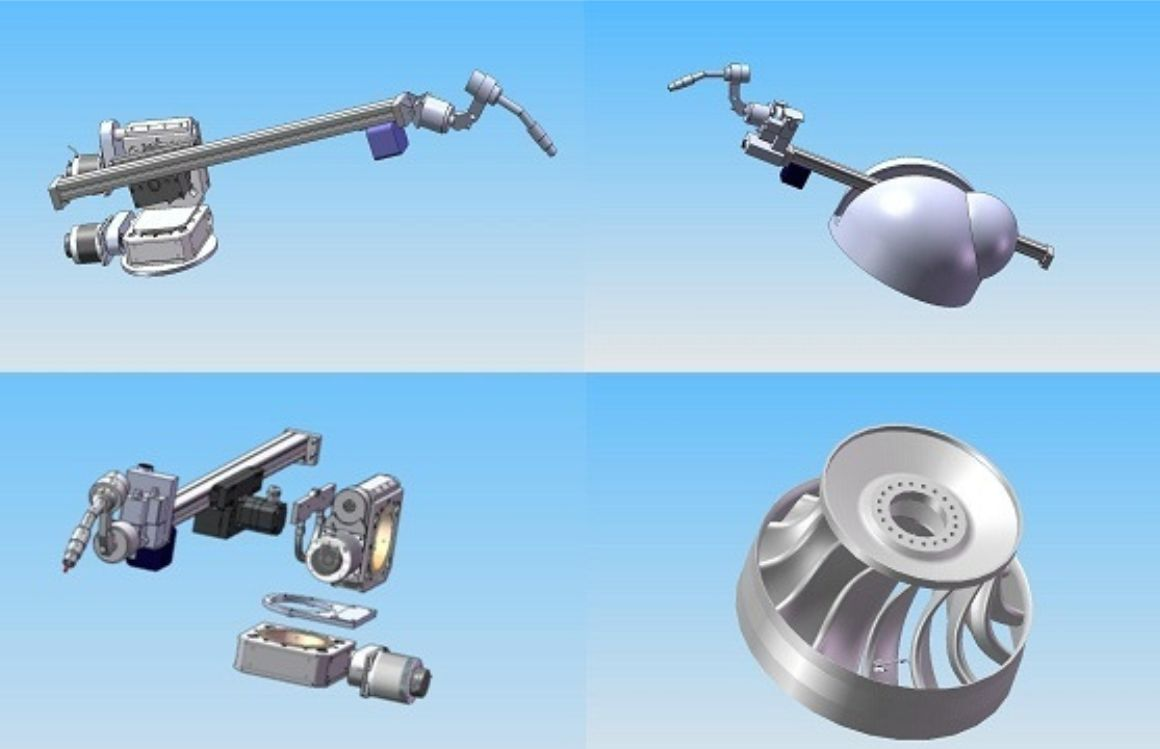
\includegraphics[width=8.4cm]{figs/esferico/esferico.jpg}
\caption{Ilustração do projeto do manipulador com base esférica.}
\label{fig:esferico}
\end{figure}

\begin{itemize}
  \item Três (3) graus de liberdade no manipulador (2R1P) e dois graus de
  liberdade no punho (2R);
  \item Mapeamento de superfície 3D com laser;
  \item Eletrônica embarcada;
  \item Soldagem por arco elétrico;
  \item Fixação nas pás por dispositivos magnéticos ou de sucção;
  \item Baixo custo;
  \item Área de trabalho em forma de anel com 2.5 m e 60 cm de altura;
  \item Peso 30 kg e dimensões 30 x 25 x 100 cm;
  \item Robô com manipulador autônomo;
\end{itemize}

O sistema robótico de manipulador com base esférica apresenta solução compatível
para a aplicação de HVOF em pás de turbinas hidráulicas, já que sua aplicação
original é soldagem das pás, semelhante ao desafio deste artigo. Todas as suas
características são vantagens e aplicam-se à solução de um sistema para HVOF.
Há, porém, desafios particulares na metalização das pás e que são desvantagens
da solução:

\textbf{Desvantagens:}
\begin{itemize}
  \item A metalização deve ser realizada em toda a pá. Portanto, o sistema
  deverá ser manualmente trocado de posição, pelo menos 4 vezes (duas posições
  para a frente e duas posições para a região de trás). E deve ser trocado de pá
  em pá;
  \item O efetuador deve percorrer a pá com grande velocidade, como exige o
  processo de metalização.
\end{itemize}